
\subsubsection{The Median Filter}
\label{subsubsection:median_filter}

The median filter is useful for denoising an image, much like the linear box filter and Gaussian filters (section \ref{subsubsection:kernels}). A median filter returns the median value of the pixel found in the application neighbourhood. This is a more complex operation than to convolve one signal with another however it can be computed in linear time \cite{cormen_2001}. It is often superior to the Gaussian filter at denoising images because it preserves edges and is not influenced by outlier intensities unlike a linear filter. In Figure \ref{fig:shot_noise} the median filter demonstrates a superior ability to remove salt and pepper noise as compared to the Gaussian filter.

\begin{figure*}[htbp]
    \centering 
    \begin{subfigure}[b]{0.3\textwidth}
        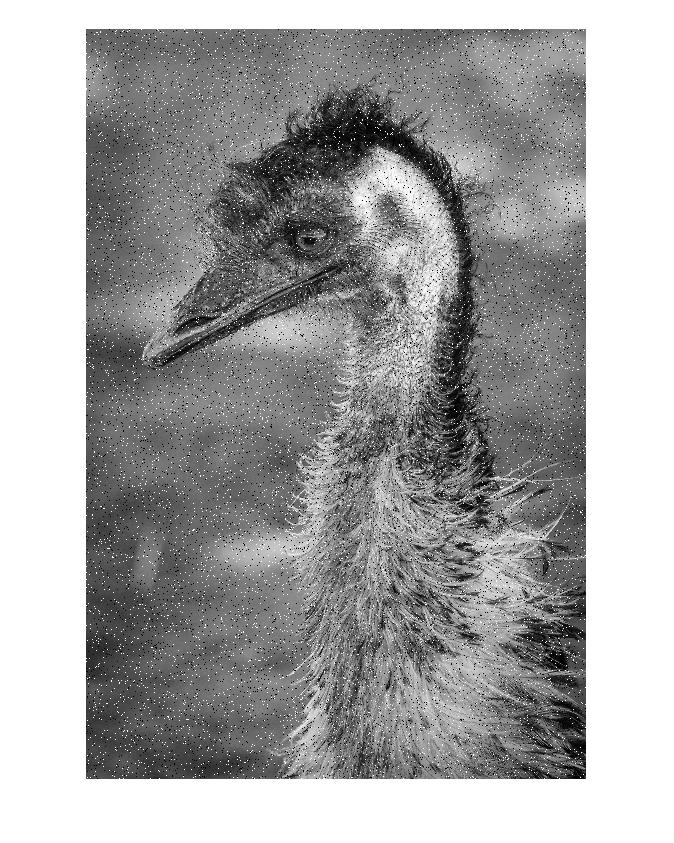
\includegraphics[width=\textwidth]{emu_noise}
        \caption{Salt and Pepper Noise}
        \label{fig:emu_noise}
    \end{subfigure}
    \begin{subfigure}[b]{0.3\textwidth}
        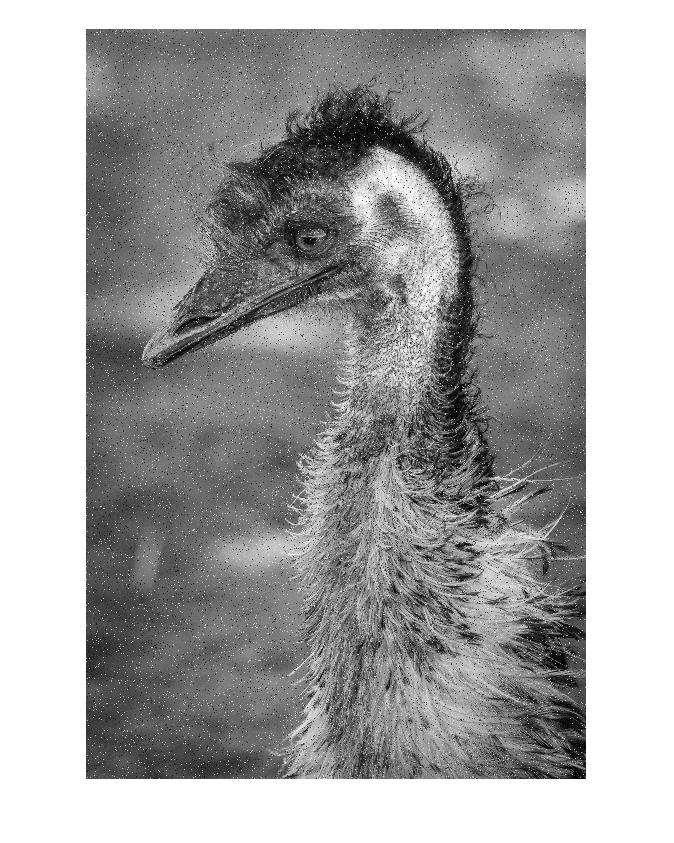
\includegraphics[width=\textwidth]{emu_gauss}
        \caption{7x7 Gaussian}
        \label{fig:emu_gauss}
    \end{subfigure}
    \begin{subfigure}[b]{0.3\textwidth}
        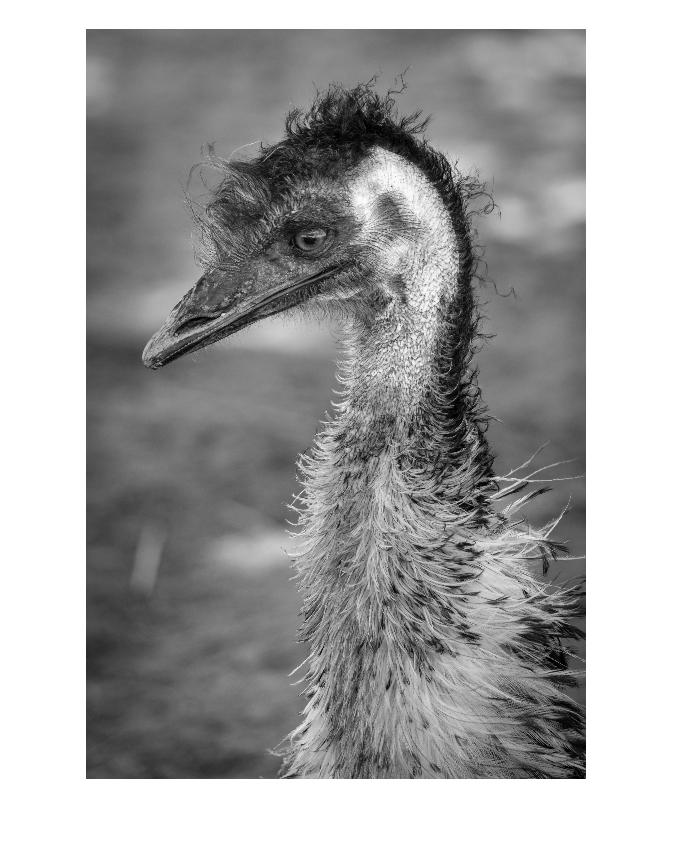
\includegraphics[width=\textwidth]{emu_median}
        \caption{7x7 Median Filter}
        \label{fig:emu_median}
    \end{subfigure}
    \captionsetup{format=hang}
    \caption{Filtering out salt and pepper noise with Gaussian and median filter. Original image by Grant Durr.}
    \label{fig:shot_noise}
\end{figure*}

Huang's Algorithm \ref{algorithm:median_filter} is one possible implementation \cite{median_filter_new}\cite{median_filter_3} of a median filter for a 2D image and is simple and of linear computational complexity, O(n). In this algorithm the histogram $H$ refers to the neighbourhood under the filter's mask. Each time the filter is moved the the histogram's leftmost column is removed and the rightmost column is added. The median is calculated for the first window position thereafter a count of the number of picture elements (pels) in a window having a value less than the current window's median is maintained. If more than half of the window's pels have a value are less than the last window's median then the median value is reduced until the number of pels with a value less than the median is greater than or equal to half of the total window pels, in this way the median value is selected. Finally the median is stored in the output image $Y$ at location $(i,j)$. 

\begin{algorithm}[H]
    \SetAlgoLined
    \KwInput{Image X of size MxN, filter size n} 
    \KwOutput{Image Y of the same size as X}
    Initialize histogram H\;
    \For{i = 1 to M}
    {
        \For{j = 1 to N}
        {
            % \For{k = $\frac{-n}{2}$ to $\frac{n}{2}$}
            \For{$k = \frac{-n}{2}$ to $\frac{n}{2}$}
            {
                Remove $X_{i+k,j-\frac{n}{2}-1}$  from H\;
                Add $X_{i+k,j+\frac{n}{2}}$ to H\; 
            }
            $Y_{i,j} \leftarrow median(H,k)$\;
        }
    }
\caption{Huang's Median Filtering Algorithm \cite{median_filter_old}}
\label{algorithm:median_filter}
\end{algorithm}